\documentclass{book}

\usepackage{fullpage}

%\usepackage{wrapfig}
%\usepackage{float}
%  \floatstyle{ruled}
%  \newfloat{callout}{thp}{lop}
%  \floatname{callout}{Things To Remember}

\usepackage{color}
\definecolor{Light}{gray}{.95}

\usepackage{amsthm}
{
  \theoremstyle{definition}
  \newtheorem{example}{Example}
}

\usepackage{graphicx}

\newlength{\calloutparindent}
\setlength{\calloutparindent}{\parindent}
%%
%% begin: the callout command
\newcommand{\callout}[3]{\label{#1}\vspace{3mm}
\begin{center}
\fcolorbox{black}{Light}{\begin{minipage}{0.85\textwidth}
    \textbf{\large Things To Remember~\ref{#1} --- #2}
    \hrule
    \vspace{2mm}
\setlength{\parindent}{\calloutparindent}
#3
  \end{minipage}}
\end{center}
\vspace{3mm}
}
\newcommand{\thingstoremember}[1]{Things To Remember~\ref{#1}}
%% end: the callout command
%%

% two chapters will precede the one here now
\setcounter{chapter}{3}

\begin{document}

\chapter{Delegation}

An important design decision when modeling data is how many Java classes to use to represent an entity. At one extreme, all of the attributes of an entity are represented by a single class, resulting in a coarse-grained design. At the other extreme, a main entity class delegates functionality to other classes, resulting in a fine-grained design.  Delegation is a very popular pattern because of the flexibility it provides. 

Programmers rarely think about memory costs when deciding how to model entities. Yet, the choices made at this design stage impact memory costs significantly. Coarse-grained designs may result in many objects with unused fields. While delegation is sometimes a way to avoid this problem, overly fine-grained data models can result in poor memory health from excessive object header overhead. This chapter explains how to evaluate object granularity design choices from a memory perspective. It begins with the costs of basic objects, and works up to examples from real applications.
  
\section{The Cost of Objects}
\label{sec:CostOfObjects}

There is no Java library method that returns the size of an object. This is by design. A Java programmer is not supposed to know either the size of an object or how it is laid out in memory.
You can obtain the exact size of objects using the HPROF agent. HPROF is enabled by the command line option: 
\ttfamily
\begin{verbatim} 
  				-agentlib:hprof=heap=dump,format=a,file=outputfile
\end{verbatim}
\normalfont
Sending a signal to the running program produces a text \textit{outputfile} with all heap objects and their sizes. Another way of obtaining an HPROF heap snapshot is using the jmap utility, which comes with your Sun JVM distribution:
\ttfamily
\begin{verbatim} 
jmap -dump:format=a,file=outputfile <pid of jvm process> 
\end{verbatim}
\normalfont
Alternatively, it is not hard to estimate the size of an object. A good estimation is usually sufficient to determine memory requirements, and make an educated choice among design alternatives. For estimating the size of an object, you need to know just a few basics, starting with the size of the Java primitive types. These are given in Table~\ref{tab:primitive-sizes}.
\begin{table}
  \centering
 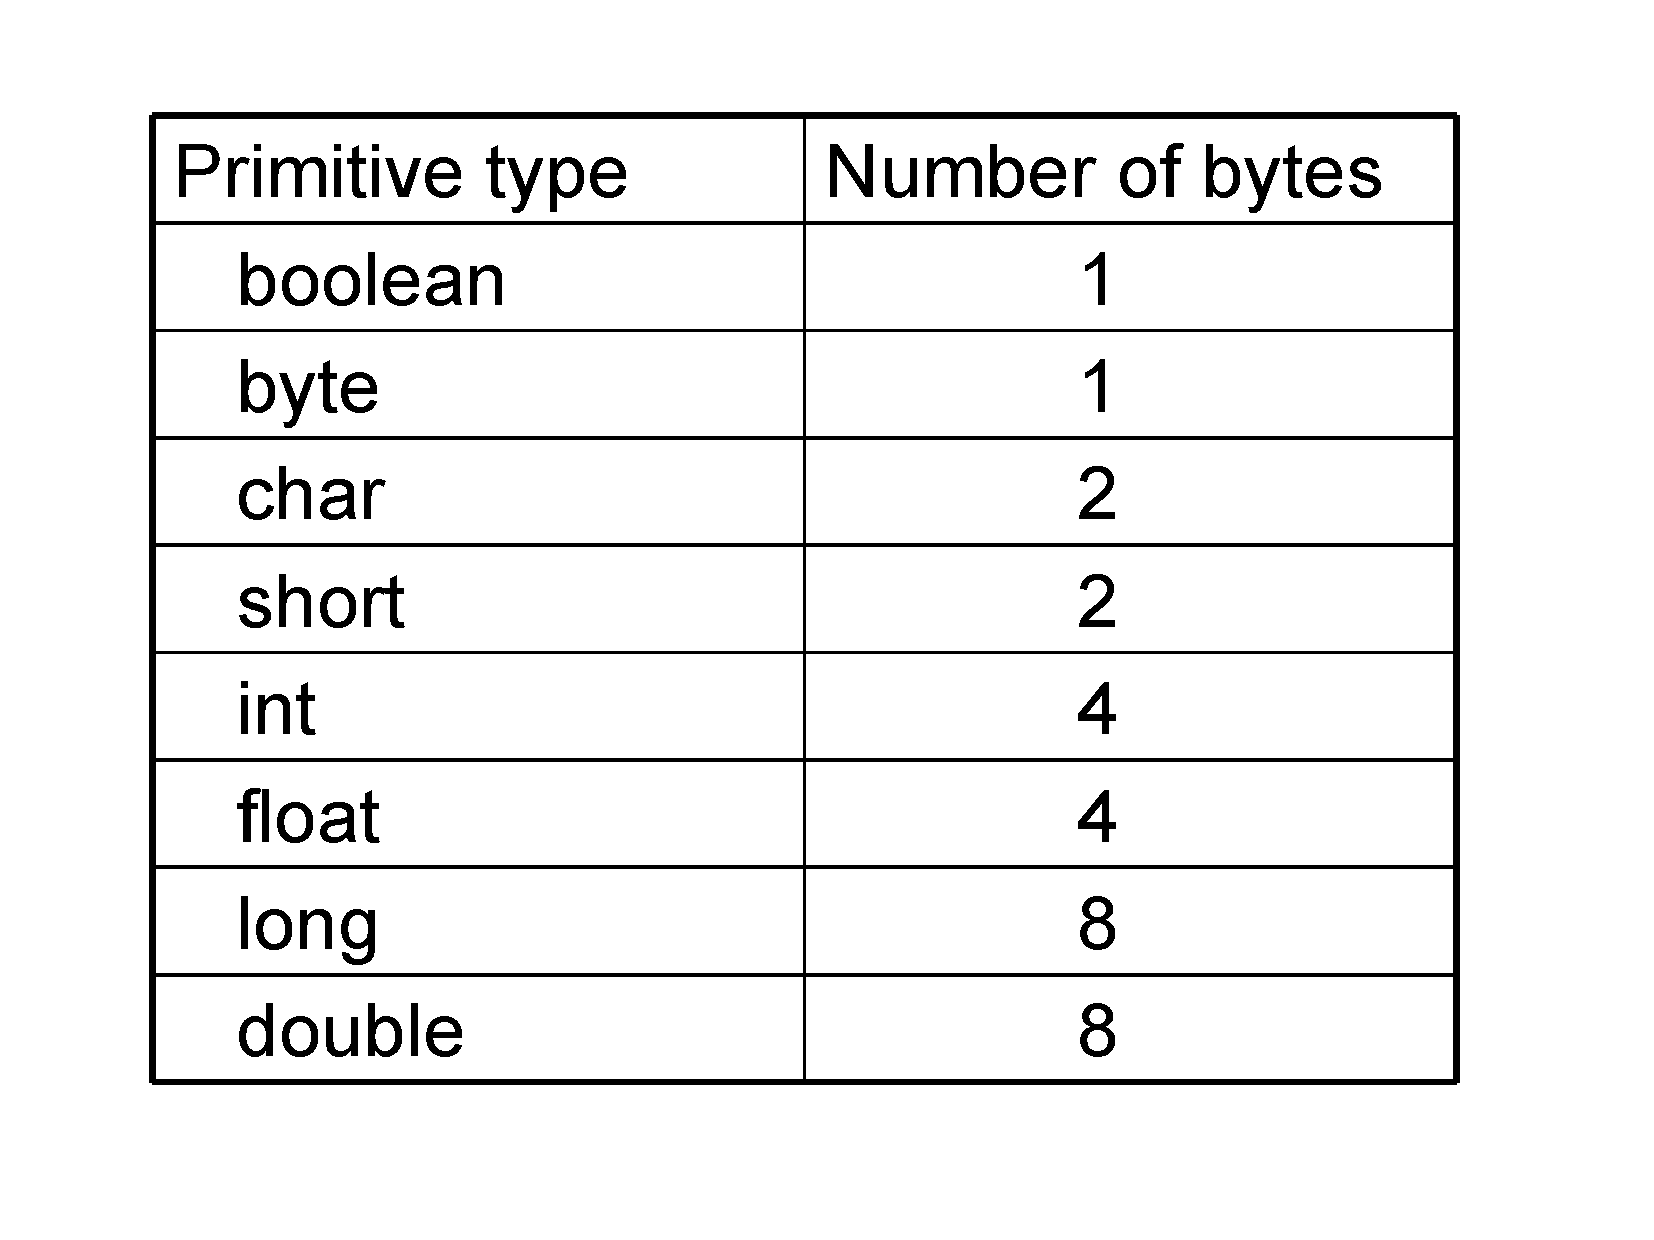
\includegraphics[width=.40\textwidth]{Figures/chapter4/primitive-byte-sizes.pdf}
 % 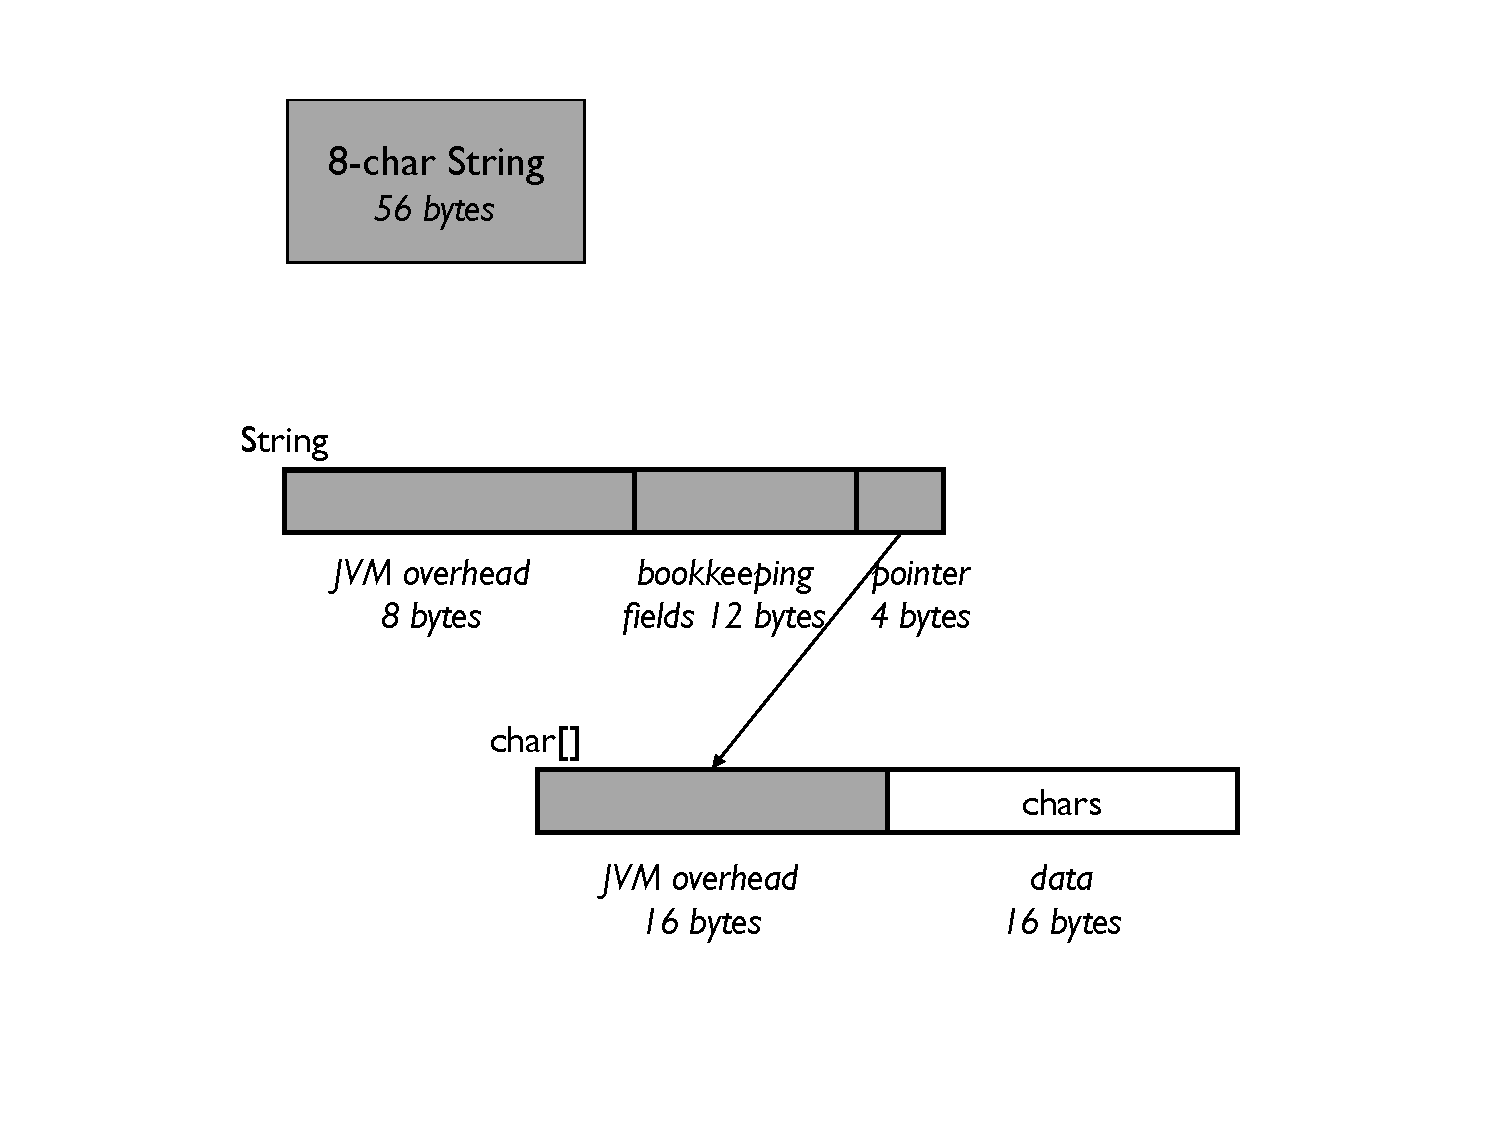
\includegraphics{eight-char-string}
  \caption{The sizes of Java primitive types}
  \label{tab:primitive-sizes}
\end{table}

Objects are much bigger. Both the JVM and the hardware impose costs, which are significant when an object is small. These costs can differ, depending on the JVM and on the hardware. Each object has a header that stores information that the JVM and garbage collector need, such as the class, a lock, and an identity hashcode. 

The underlying hardware can impose alignment costs. The hardware may require 2-byte, 4-byte, or 8-byte alignment, depending on the type of the data. For example, integers are usually aligned on a 4-byte boundary, and some hardware might require a double to be aligned on an 8-byte boundary. A JVM may impose an alignment requirement above and beyond the hardware, if there is some performance benefits for storage allocation and garbage collection. 

To show how different JVMs vary, numbers here are given for both the SUN Java 6 (update 14)JVM and the IBM Java 6 (J9 SR4) JVM. These numbers are for 32-bit architectures. Keep in mind that these numbers are subject to change in future JVM releases, but it is useful to have concrete examples.
   
The Sun JVM allocates 8 bytes per object header, and the IBM JVM allocates 12 bytes per header. For array objects, the header has an additional integer to store the number of array elements. An array header size is 12 bytes for the Sun JVM, and 16 bytes for the IBM JVM. Both JVMs allocate objects on 8-byte boundaries. This means that the size of an object is a multiple of 8. For both JVMs, the smallest that an object with at least one byte of data can be 16 bytes. 
The table~\ref{tab:boxed-scalar-sizes} gives the resulting sizes for boxed scalars.

\begin{table}
  \centering
 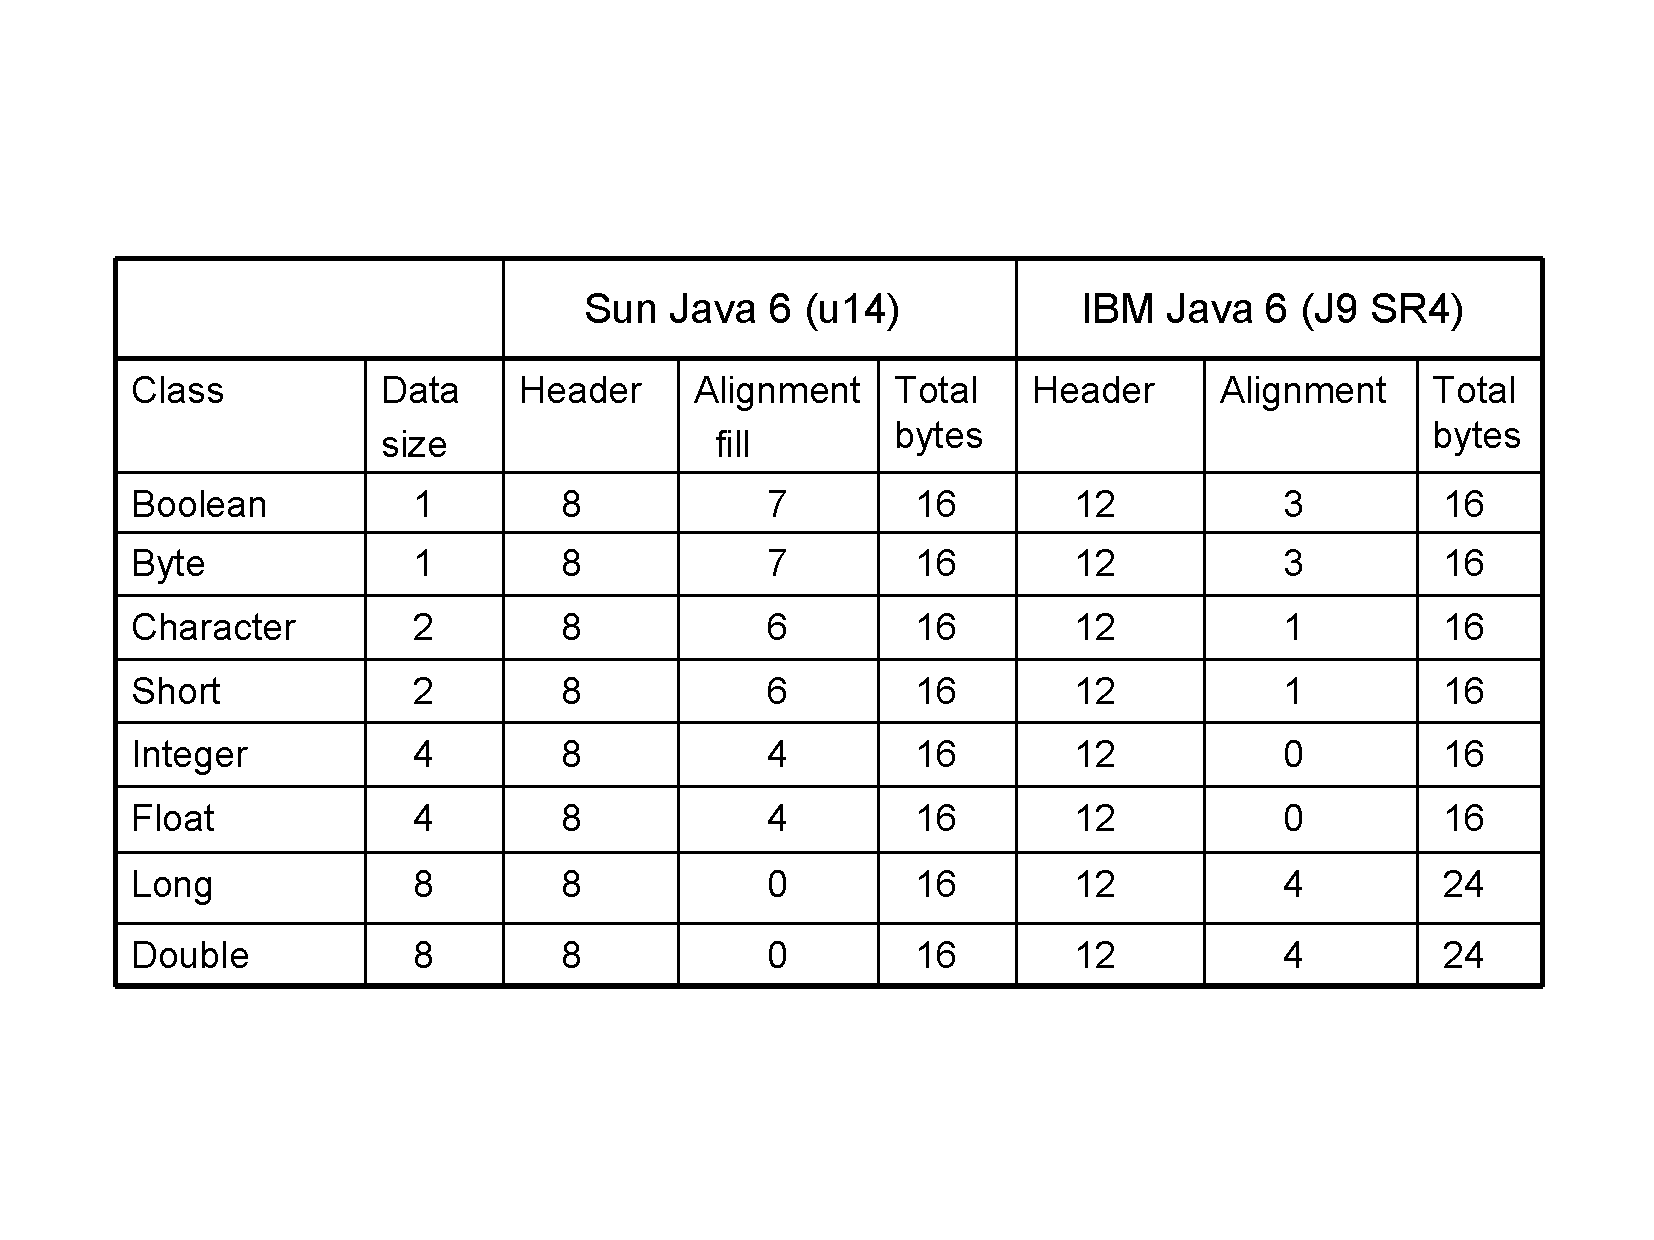
\includegraphics[width=.60\textwidth]{Figures/chapter4/boxed-scalar-sizes.pdf}
 % 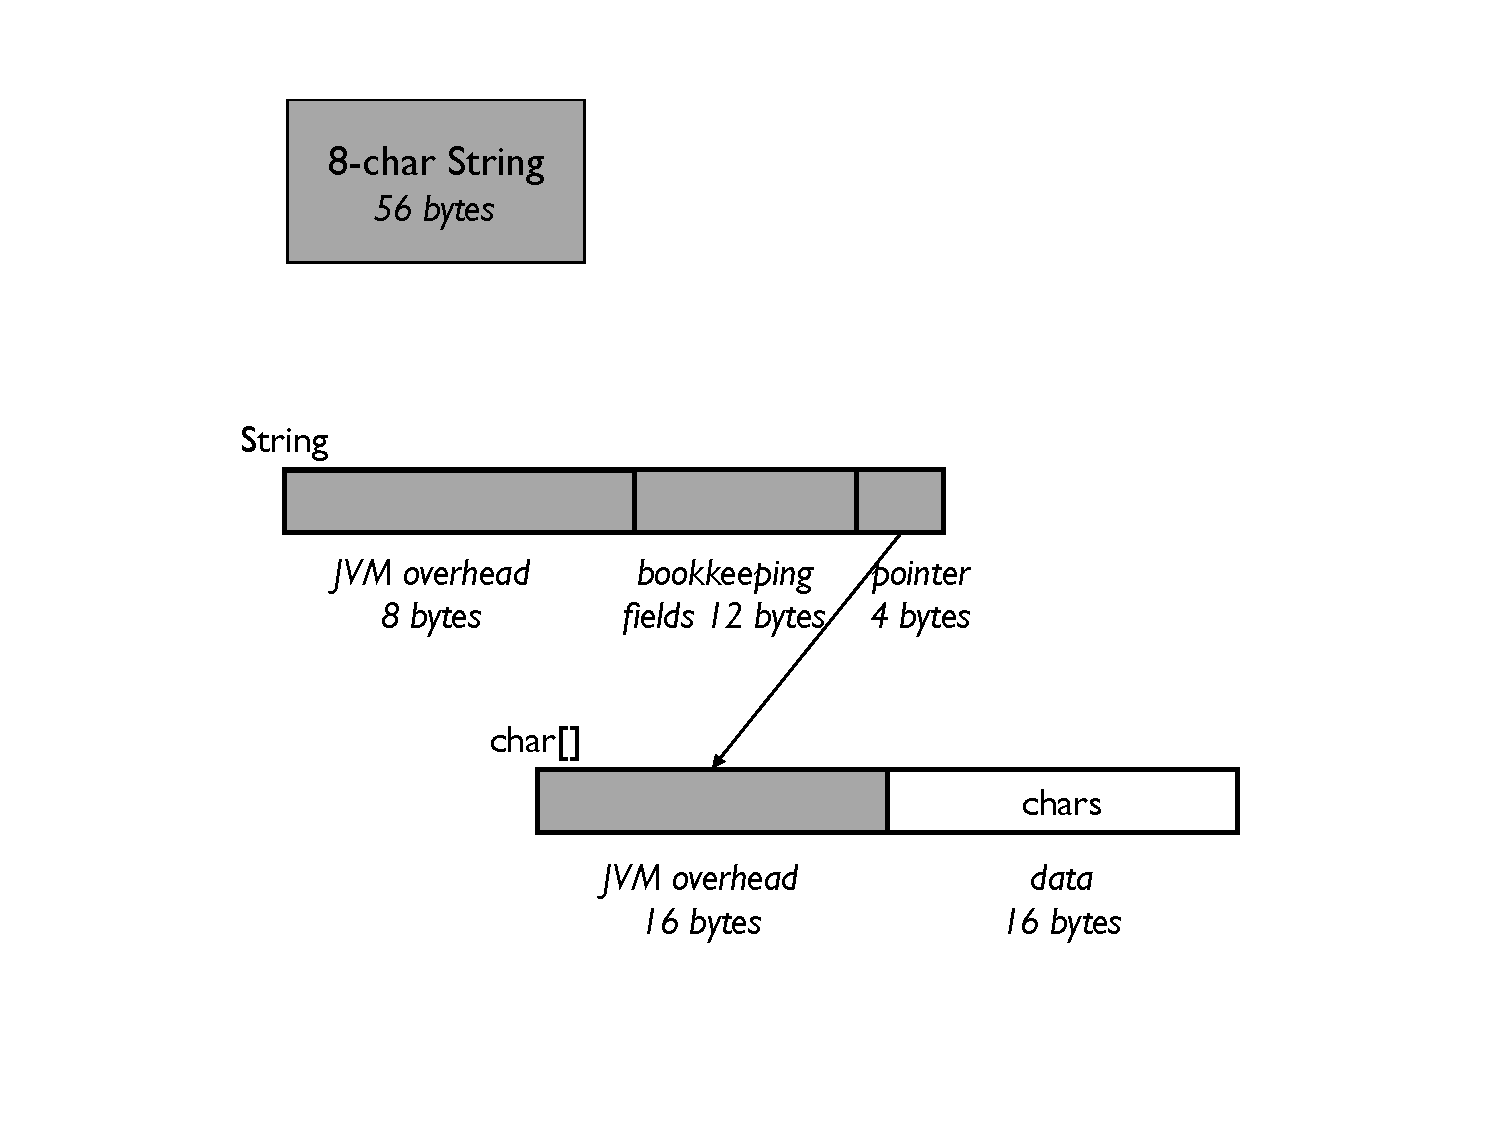
\includegraphics{eight-char-string}
  \caption{The sizes of boxed scalar objects.}
  \label{tab:boxed-scalar-sizes}
\end{table} 

There is a simple rule that holds here. The size of the object is obtained by adding together the size of the header and the data, and then rounding it up to the nearest multiple of 8. The generalization of this rule gives you a good way to estimate the size of any object. Often, this estimate turns out to be the real object size, but not always. The JVM has freedom in the way it lays out an object. 
 
\callout{callout:object-size-estimation-rule}{Minimum Size Estimation Rule}{
    Let $Header$ be the size of an object header required by the JVM, and $Alignment$ be the object alignment. That is, every object must be allocated at an address which is a multiple of $Alignment$. You can estimate the size of an object by 1) summing up the sizes of all of the data stored in the object, including data from superclasses, 2) adding this sum to $Header$, and 3) rounding the result up to the next multiple of $Alignment$. 
    
	This rule computes the minimum size of an object. The calculation is exact if the JVM packs and rearranges fields to fit into the smallest space.
}


\begin{example}[Class with primitive fields.]
Consider an \texttt{EmployeeStatus} class with all primitive fields:

\ttfamily
\begin{verbatim} 

			class EmployeeStatus {
        int hoursPerWeek;
        boolean exempt;
        double salary;
        char jobCode;
        int yearsOfService;
			}
\end{verbatim}
\normalfont
Applying the object size estimation rule, assuming both $Header$ and $Alignment$ are 8 bytes, the minimum size of an \texttt{EmployeeStatus} object is 32 bytes. You first add primitive sizes 4+1+8+2+4 (=19), add in the header size 8 (=27), and then round to the next multiple of 8. The result is 32 bytes.  If the header is 12 bytes, the estimated size is also 32 bytes, since 19+12 is 31, which again rounds up to 32. The overhead consists of the object header and the alignment bytes. You can compute the bloat factor of this object by subtracting the data size from the total size to obtain the overhead size, and then dividing this overhead by the total size.  The bloat factor is 40.6\%.

How accurate are these estimates for the two JVMs?  For the Sun JVM, an \texttt{EmployeeStatus} object is 32 bytes. The minimum size estimation rule works well here, since the Sun JVM does a good job packing fields. For the IBM JVM, an \texttt{EmployeeStatus} object is 40 bytes. It turns out that the IBM JVM does not pack fields that are less than 4 bytes. In other words, the IBM JVM aligns all fields on 4 byte boundaries. When an object has several fields that are less than 4 bytes, such as booleans and chars, then the rule may underestimate its size.
			
\end{example}

Estimating total memory usage starts with determining the size of each object type. The \texttt{EmployeeStatus} example shows that the sizes can vary, depending on the JVM. Not only do different JVMs layout objects differently. A new version of a JVM may change its layout algorithm. In most cases, a good estimate of object sizes is sufficient, so that it is usually not necessary to worry about these variations among the JVMs. The minimum size estimation rule is simple and accurate most of the time.

\section{The Cost of Delegation}

The \texttt{EmployeeStatus} class is not a very realistic example, since it has only primitive fields. Usually, a class has fields that are objects. Here is a more realistic \texttt{EmployeeStatus} class, with several object fields. An employee has a name, which is a \texttt{String}, and a start date, which is a \texttt{Date}. The type of \texttt{salary} has been changed from \texttt{double} to \texttt{BigDecimal}. \texttt{BigDecimal} avoids potential roundoff errors.
\ttfamily
\begin{verbatim} 
			class EmployeeStatus {
        int hoursPerWeek;
        String name;
        BigDecimal salary;
        Date startDate;
        boolean exempt;
        char jobCode;
        int yearsOfService;
			}
\end{verbatim}
\normalfont
 
In Java, an object field is implemented as a \textit{delegated} object, that is, as a separate object pointed to by the owner object. On 32-bit architectures, a pointer is 4 bytes. You can estimate the size of an object using the object size estimation rule, where a pointer field is 4 bytes. For example, for \texttt{EmployeeStatus}, add the field sizes 4+4+4+4+1+2+4 (=23), add in 8 bytes for the header (=31), and then round this up to 32 bytes. 

The memory layout for an employee "John Doe" is shown in Figure~\ref{employee-status}. There are five objects, occupying 144 bytes.
 \begin{figure}
  \centering
 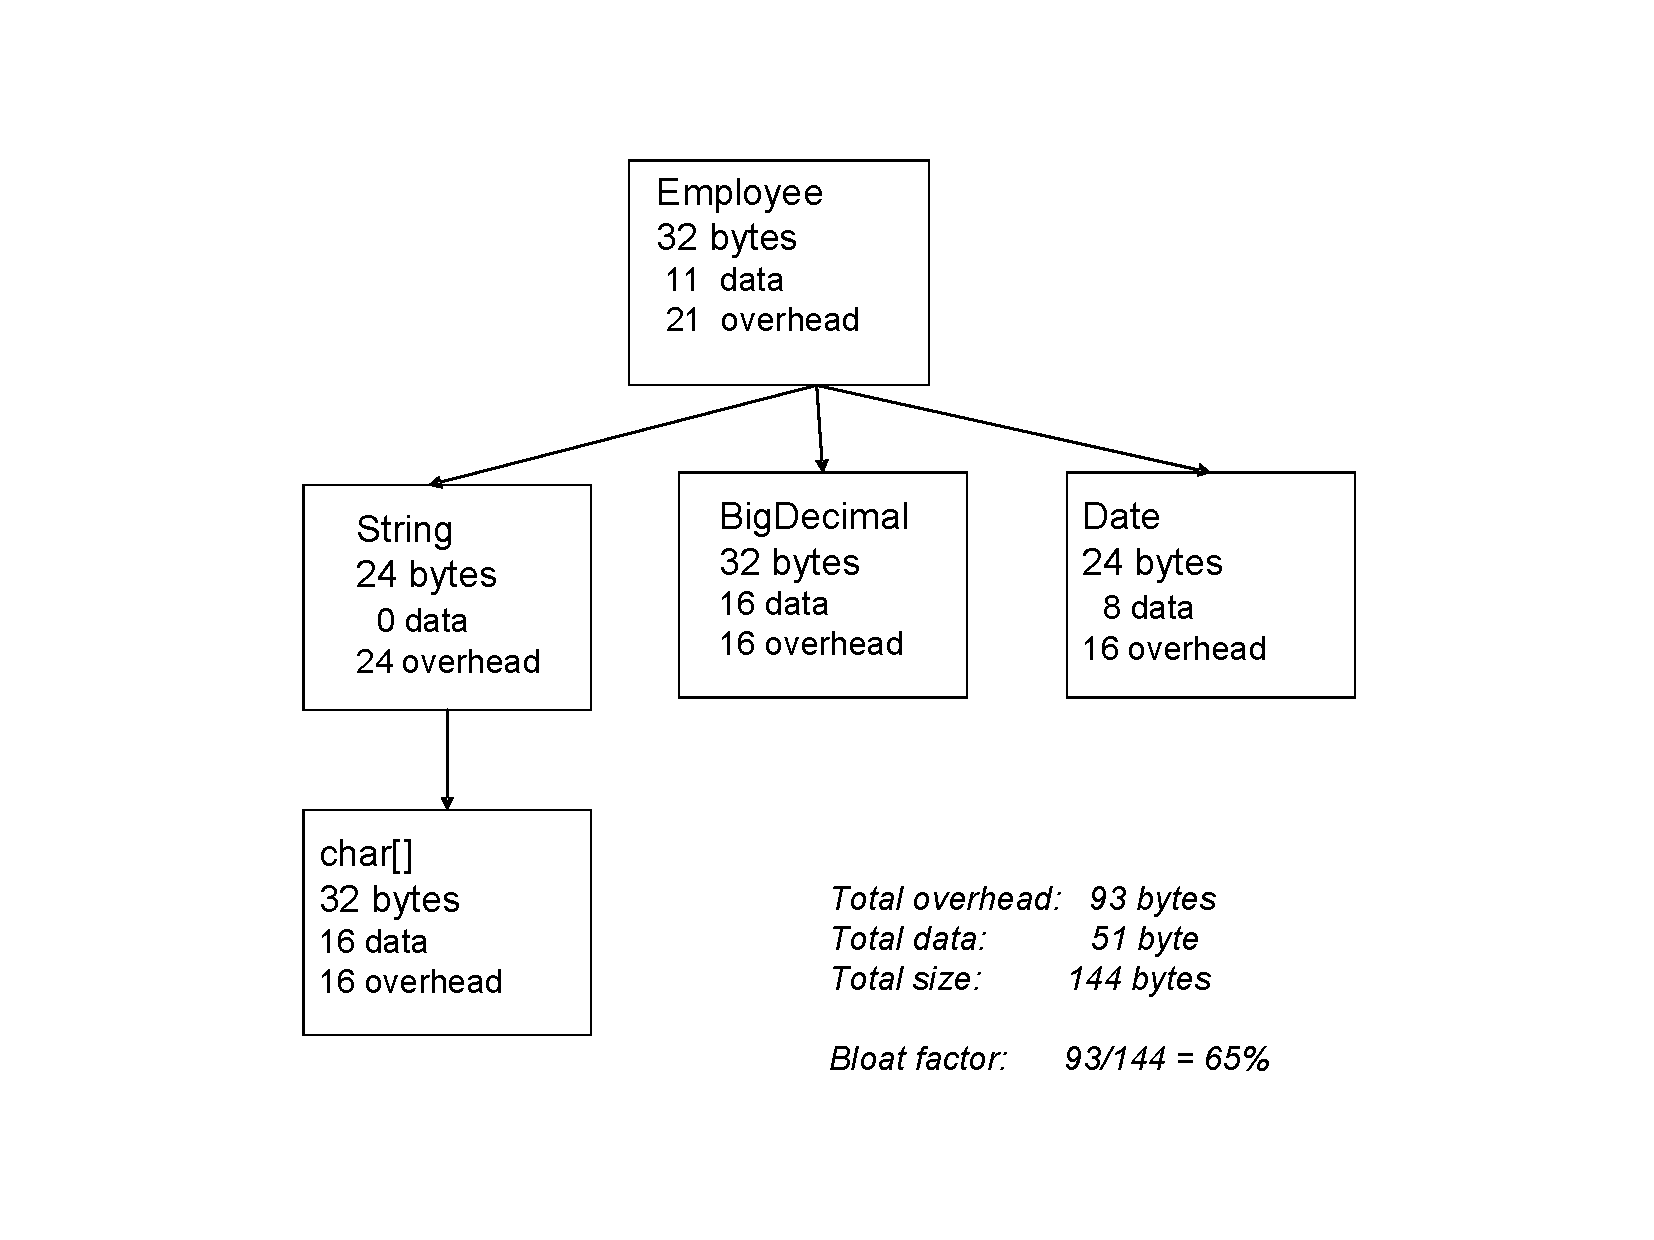
\includegraphics[width=.60\textwidth]{Figures/chapter4/employee-status.pdf}
 % 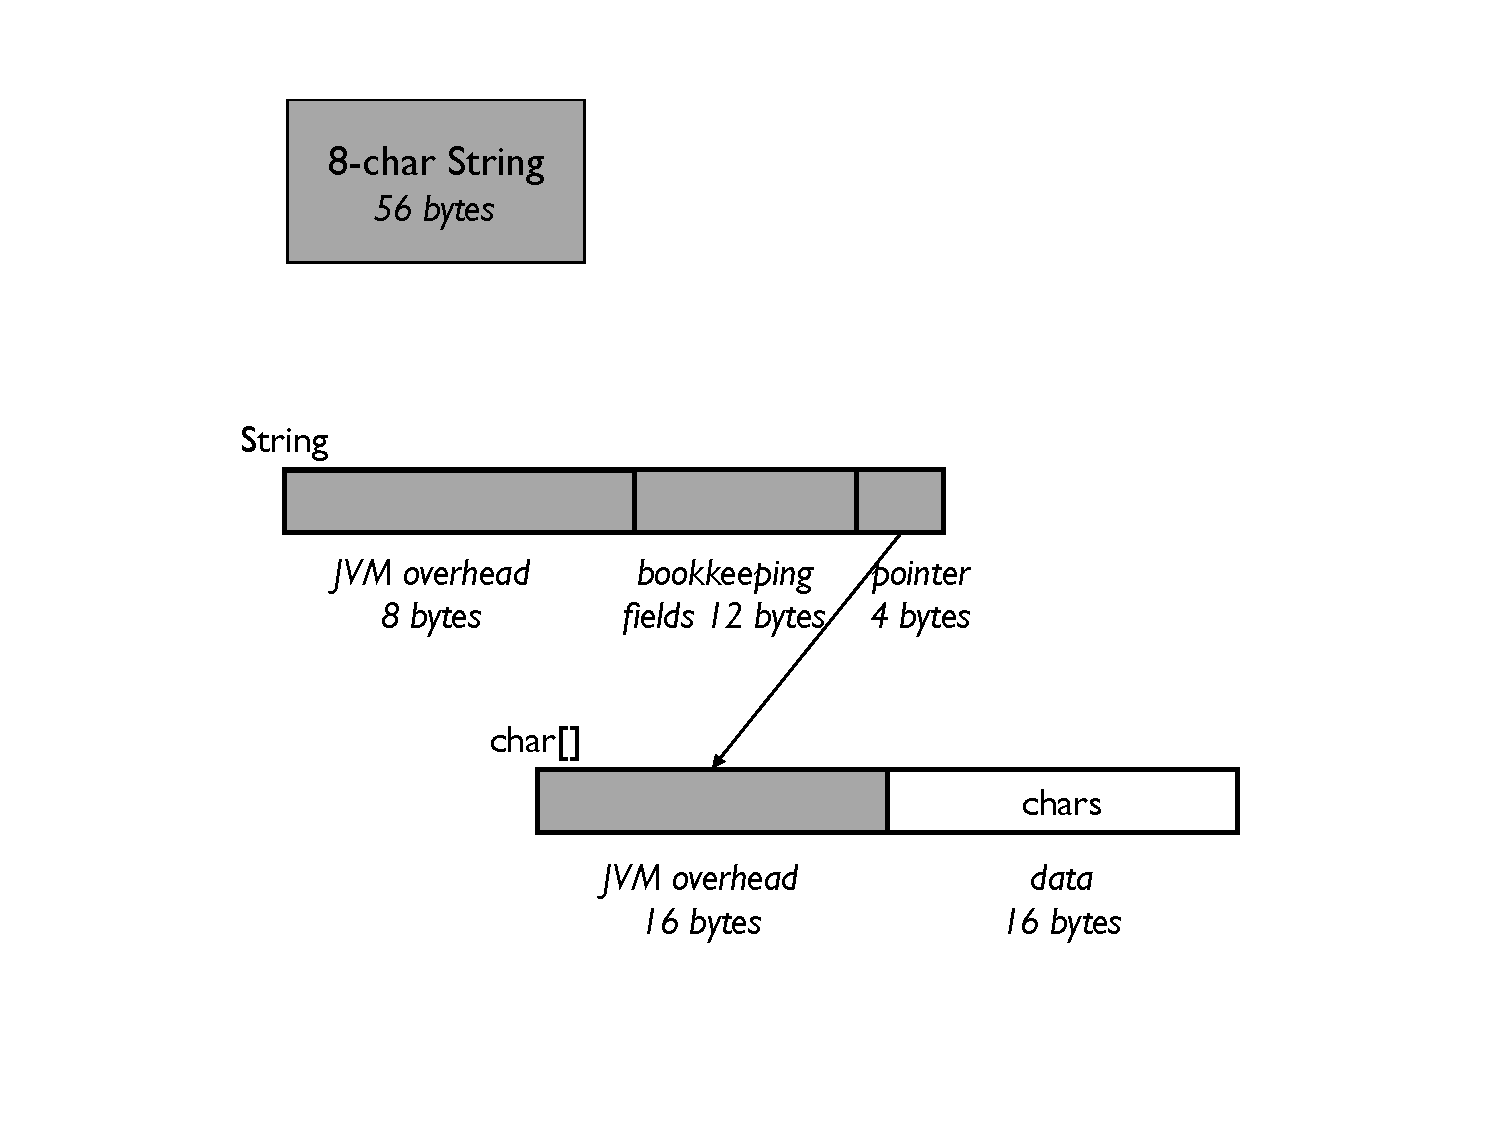
\includegraphics{eight-char-string}
  \caption{The memory layout for an employee "John Doe"}
  \label{fig:employee-status}
\end{figure}

Comparing the total size of these objects with the original \texttt{EmployeeStatus} size in Section~\cite{CostOfObects}, you see that the storage has more than quadrupled. In the new version, there are 51 bytes of real data, and 93 bytes of overhead. The bloat factor is now 65\%. As this example shows, delegation increases memory bloat because there is an additional object header and pointer for each delegated object. Delegation may also force additional alignment costs, since each new delegated object has to be aligned to an 8-byte boundary. 

What else contributes to the overhead in Figure~\ref{fig:employee-status} besides delegation?  First, the entire \texttt{String} object is overhead. Recall from Section~\ref{sec:MemoryBloatFactor} that a \textbf{String} is two objects, a wrapper and a \texttt{char} array, and only the \texttt{char} array has actual data in it. Secondly, there are some null pointer fields, and alignment bytes. Finally, object header of \texttt{EmployeeStatus} also contributes to the overhead.

In the spirit of keeping things simple, Java does not allow you to nest objects inside other objects. You cannot build a single object out of other objects. That is, you cannot nest an array inside an object, and you cannot store objects directly in an array.  You can only point to other objects. Even the basic data type \texttt{String} consists of two objects. This means that delegation is pervasive in Java programs, and it is difficult to avoid a high level of delegation overhead. Single inheritance is the only language feature that can be used instead of delegation to compose two object, but single inheritance has limited flexibility.  In contrast, C++ has many different ways to compose objects. C++ has single and multiple inheritance, union types, and variation. C++ allows you to have \texttt{struct} fields, you can put arrays inside of structs, and you can also have an array of structs.  

In Java, delegation is one of the costs you pay for basic object-oriented programming. This cost is often considered to be insignificant. Delegating to another object is just a single level of indirection. But the costs of the pointers and object headers needed to implement delegation add up quickly, and contribute significantly to large bloat factors in real applications.

\section{Fine-Grained Data Models}
\label{fine-grained-data-models}

The Java language makes it hard to avoid delegation. Programmers can make design decisions that lead to even more delegation. 
The current software engineering culture tends to promote delegation, and for good reasons. Delegation provides a loose coupling of objects, making refactoring and reuse easier later on. Delegation is also more elegant than single inheritance, especially if the base class has a lot of extra baggage that the subclass does not need. In languages with single inheritance, once you have used up your inheritance in your single inheritance hierarchy, it becomes hard to refactor your code. In this case, delegation is more flexible than inheritance for specializing types. However, it is possible to overuse delegation, resulting in an overly fine-grained data model with many small objects. Fine-grained data models can be expensive both in execution time and memory space. 

There is no simple rule that can always be applied. Each situation has to be evaluated in context, and there may be tradeoffs among different goals. To make an informed decision, you need to determine the impact of delegation on memory requirements, by measuring the object sizes and overhead.  

 
\begin{example}[Employee emergency contact] 
This is an example of a highly delegated design, what not to do. This kind of poor design may seem contrived, but it is not uncommon in real applications. Often programmers are not aware the overhead that delegation introduces.

In this example, an emergency contact is added to the \texttt{EmployeeStatus} class. An emergency contact is a person and a preferred method to reach her.  The preferred method can be email, cell phone, work phone, or home phone. All contact information is stored with the contact person, just in case the preferred way does not work in an actual emergency. Here are class definitions that model an emergency contact for an employee. The memory layout with costs for these classes is shown in Figure~\ref{fig:employee-status-fine-grained}.
\ttfamily
\begin{verbatim} 
			class EmployeeStatus {
        ...
        EmergencyContact contact;
			}
			
			class EmergencyContact {
				ContactPerson contact;
				Contact preferredContact;
			}
			
			class ContactPerson {
				String name;
				String relation;
				EmailAddress email;
				PhoneNumber phone;
				PhoneNumber cell;
				PhoneNumber work;
			}
			
			class Contact {
				ContactPerson owner;
			}
			
			class PhoneNumber extends Contact {
			  char[] phone = new char[10];
			}
			
			class EmailAddress extends Contact {
				String address;
			}
			
			class Address extends Contact {
				String address;
			}
			
\end{verbatim}
\normalfont
 \begin{figure}
  \centering
 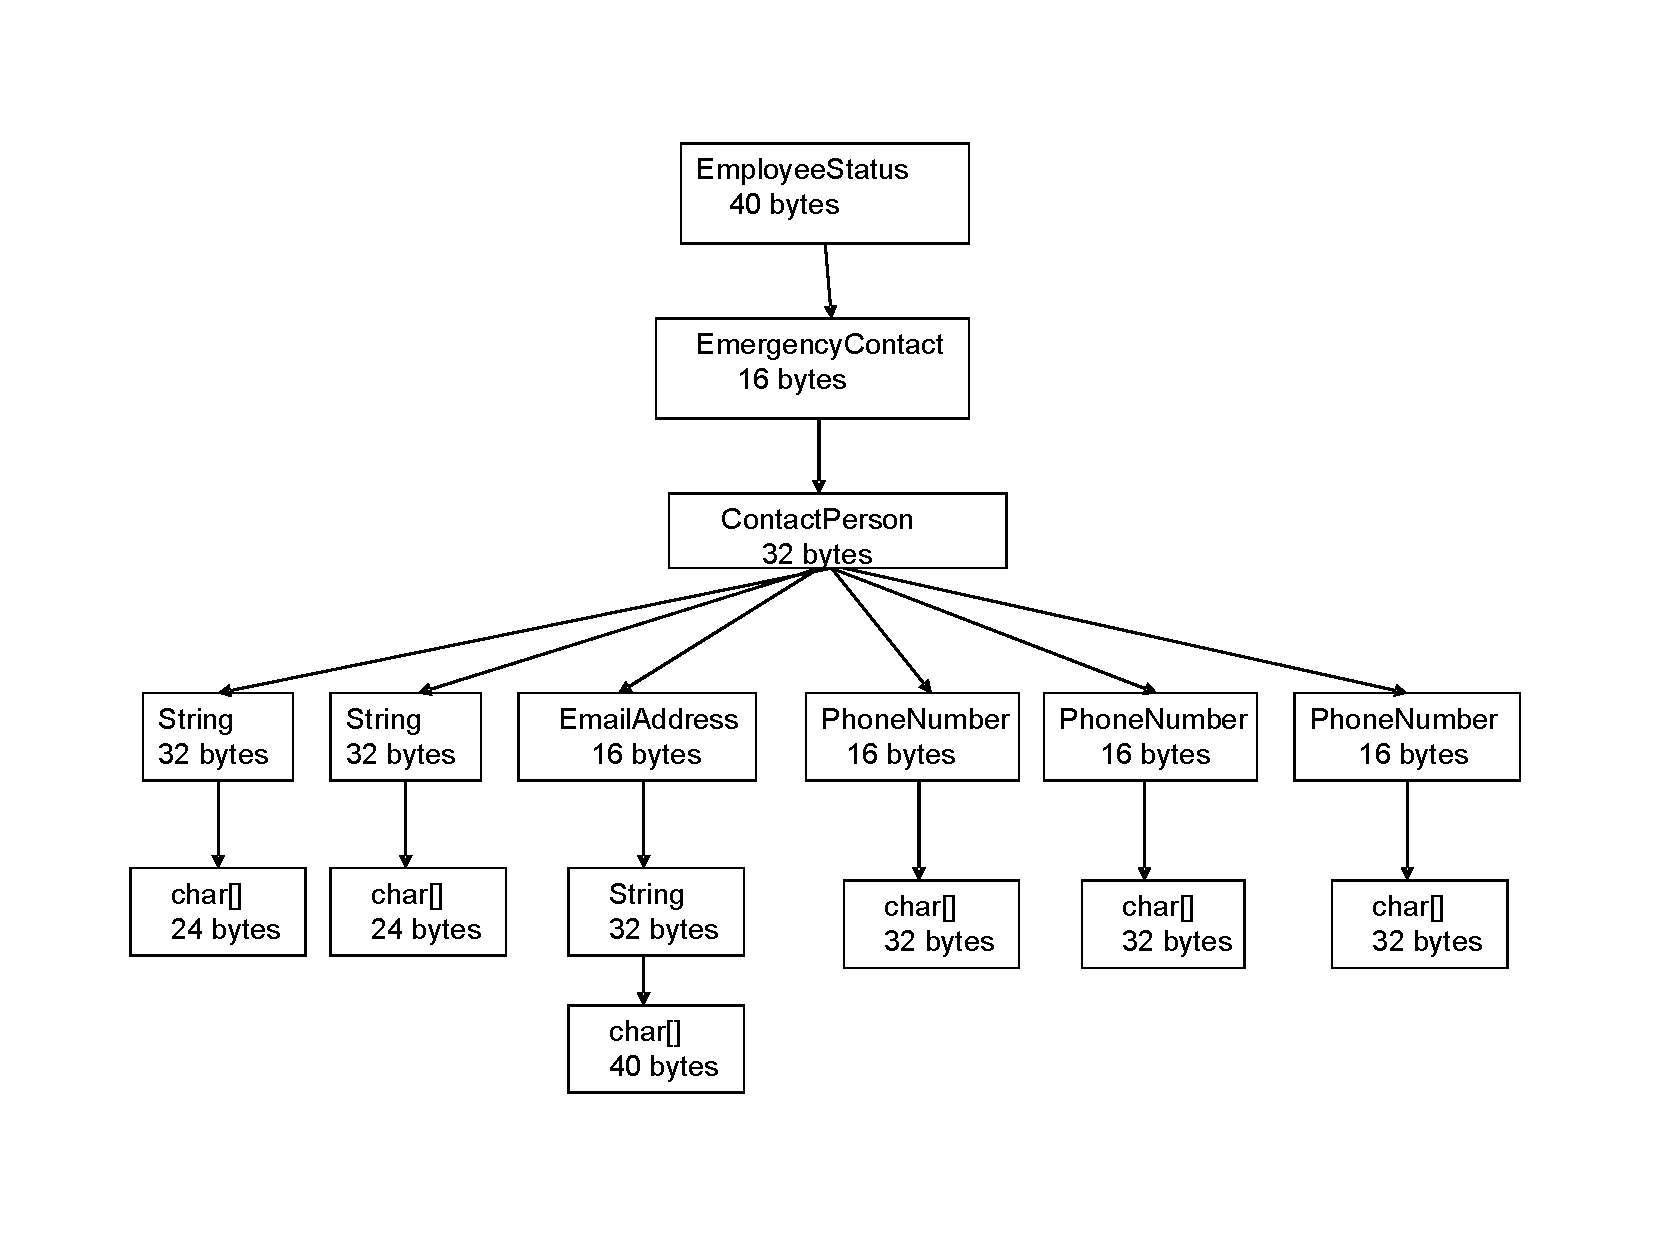
\includegraphics[width=.70\textwidth]{Figures/chapter4/employee-status-fine-grained.pdf}
 % 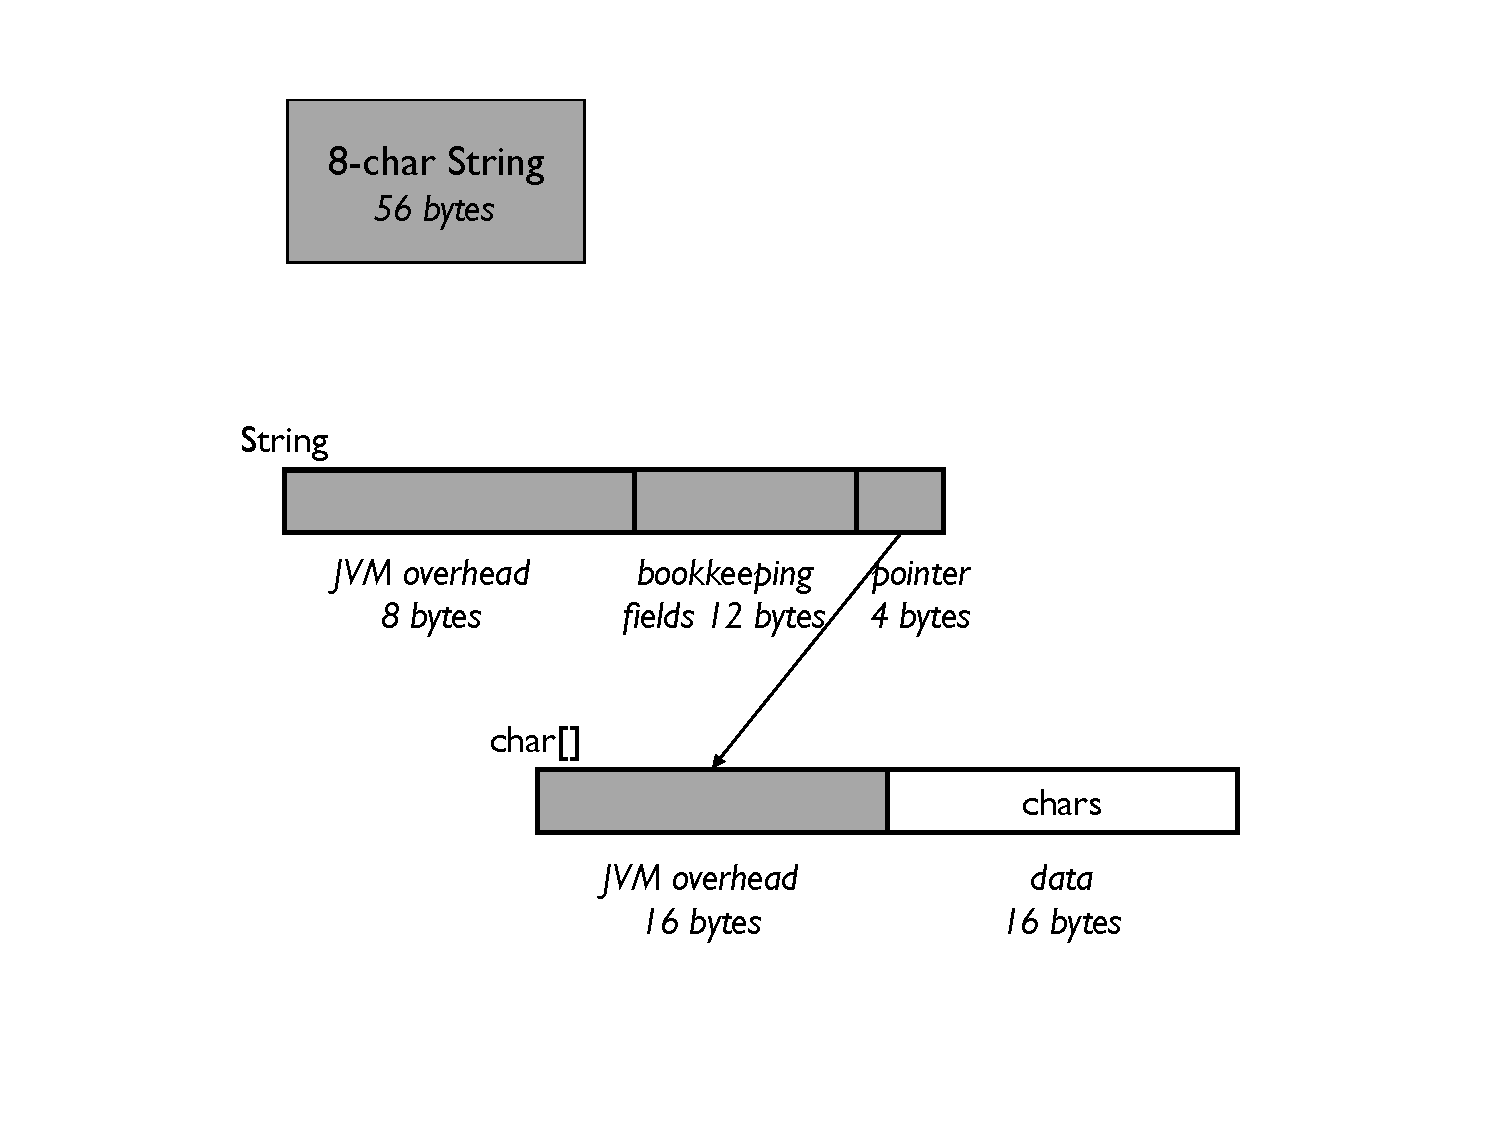
\includegraphics{eight-char-string}
  \caption{The memory layout for an employee with an emergency contact.}
  \label{fig:employee-status-fine-grained}
\end{figure}

In this figure, there are 15 delegated objects, just to store emergency contact information. This seems like too many objects, and it should be possible to design a more compact the representation by eliminating some of the delegation. One object that looks superfluous is \texttt{EmergencyContact}, which encapsulates the contact person and the preferred contact method. You can eliminate one level of delegation by inlining the two \texttt{EmergencyContact} fields in the parent \texttt{EmployeeStatus} object, and then eliminating the \texttt{EmergencyContact} object altogether. Alternatively, it makes more sense to move the \textbf{ContactPerson} field to the EmployeeStatus object, and the \texttt{preferredContact} field to the \texttt{ContactPerson}, since the preferred contact method is really an attribute of the contact person. Here is the modified code:
\ttfamily
\begin{verbatim}
	class EmployeeStatus {
        ...
        ContactPerson contact;
			}
			
			class ContactPerson {
				String name;
				String relation;
				EmailAddress email;
				PhoneNumber phone;
				PhoneNumber cell;
				PhoneNumber work;
				Contact preferredContact;
			}
\end{verbatim}
\normalfont
This change eliminates an object, but not much space. You can save considerably more space by inlining the four \texttt{Contact} objects into the \texttt{ContactPerson} object. This results in a 17\% total space reduction. In a system with many in-memory \texttt{EmployeeStatus} entities, this reduction is significant. To make this change, you need to somehow encode the preferred contact method in \texttt{ContactPerson}.  There are several ways to do this. One way is to use an enumerated type field to discriminate among the different contact methods:
\ttfamily
\begin{verbatim} 
      enum PreferredContactMethod {
         EMAIL, HOME_PHONE, CELL_PHONE, WORK_PHONE;
      }
      
       class ContactPerson {
        PreferredContactMethod preferred;
        String name;
        String relation;
        String email;
        char[] cellPhone;
        char[] homePhone;
        char[] workPhone;
      }		
\end{verbatim}
\normalfont
Another way to indicate the preferred contact method is to specialize the \texttt{ContactPerson } using inheritance:
\ttfamily
\begin{verbatim}
     class EmailContactPerson extends ContactPerson {
              ....
     }
     class CellPhoneContactPerson extends ContactPerson {
              ....
     }    
     class HomePhoneContactPerson extends ContactPerson {
              ....
     }    
     class WorkPhoneContactPerson extends ContactPerson {
              ....
     }    
\end{verbatim}
\normalfont    
By specializing the \texttt{ContactPerson} through inheritance, you do not need a field in \texttt{ContactPerson}, like \texttt{preferred} or \texttt{preferredContact}, so this seems to be the better solution from a memory perspective. However, using inheritance has some traps. In this example, the user has to know which contact method is preferred in order to create the \texttt{ContactPerson} object. This information may not be available. Using inheritance here is less flexible than using the enumated type field.
\end{example}
When many objects are used to represent a single entity, this is an indication that the data model is using too much delegation. For example, using 15 objects to represent the emercency contact information seems high. Often, a design with fewer, bigger objects is cleaner, has less overhead, and is more scalable. 

\section{Large Base Classes}

There is one scenario where inheritance seems clearly to be a good choice. This is when there is a cross-cutting feature, common to many objects. In this case, adding the feature to a base class is a good solution. All objects that require this feature can inherit from the base class. 


\begin{example}[Keeping track of updates] 

A common requirement in data management is to keep track of update information, that is, when was a record last updated and by whom. Here is a base class that stores update information: 
\ttfamily
\begin{verbatim}
      
\end{verbatim}
\normalfont

\end{example}

Usually, objects in a highly delegated design are small. A problem arises when there are too many of these objects, which leads to a high bloat factor.  Too many big objects is an even worse problem. This can happen when large base classes are used in a highly delegated design. The fields in a base classes are inherited in every single object in large delegated structure, so costs quickly multiply.
\section{64-bit Architectures}

n th 64-bit world, that string is now 96 bytes, and the reason is 50\% larger than it was in 32-bit JVM. The reason is first of all So in this case, just the delegation costs is now 32 bytes, which is basically 1/3 of the cost, and the total cost of the string is up by 50\%.  In general, this is a real problem for fine-grained designs. Unfortunately, a lot of designs out there are fine0grained, and we'll see the reasons for that. 


So just lets talk a little about what this means for 64-bit JVMs. People are busting out of this 32-bit address space now, and they are saying let's go to 64-bit, and that will solve everything. Unfortunately, when you go to 64-bit, things blow up pretty quickly. , the object headers are double, pretty sure that's the same thing in sun. arrays are not quite double. 24 bytes. The other thing is that all the pointers instead of being 4 bytes, are now 8 bytes; and finally, there's still that same alignment cost in J9. In SUN you will have a higher alignment cost, since in SUN now it's aligned to 8-byte boundary, where it was aligned to 4-byte boundary before.  The studies I've read, both outside and inside IBM, are showing that going to a 64-bit JVM will increase your memory usage by 40-50\%, and I've heard arguments that say that yur application will run faster, because of the native architecture and all that,  but in some cases there is evidence that it may run slower, because of the worse cache locality. It's another example where it's super important to measure, and not make assumptions that this will fix my speed problem, or it will fix my memory problem. There are a lot of surprises in this area. So J9, and some of the other JVMs, I don't think SUN has this yet, I coud be wrong, I know JRocket has it , they have a mode have called compress addressing, where they can squeeze a few extra bits out of the 32-bit addresses, and in J9 6SR2 is going to allow addressing of up to 28 gig with a 32 bit address still, so without all of these additional footprint problems, if you use this compressing flag. From what I've read, it's only a few percentage degradation in performance, it's pretty minor, so it can certainly help people in this transition area.




\section{Summary}


\end{document}
